%\documentclass[12pt]{article}
%\usepackage[a4paper, margin=1in]{geometry} 
%\usepackage{graphicx} 
%\usepackage{hyperref}
%\usepackage{float}
%\usepackage{multicol}
%\usepackage{multirow}
%\usepackage{amsmath}
%\usepackage[font=small, labelfont=bf]{caption}
%
%\begin{document}

%
% Introduction to phylogenetic trees
%
\subsection{Introduction to phylogenetic trees}
A phylogenetic provides additional views on the analysis of multiple sequences.

%
% Elements of phylogenetic tree
%
\subsubsection*{Elements of phylogenetic tree}
\begin{itemize}
\item Terminal nodes: sequences, gruops of genes, species, operational taxonomic units
\item Internal nodes: hypothetical ancestral units
\item Edges: often represent distances
\end{itemize}

%
% Types of trees
%
\subsubsection*{Types of trees}
\begin{itemize}
\item Cladogram or phylogram
\item Bifurcating or multifurcating
\item Rooted or unrooted
\end{itemize}

\begin{figure}[H]
  \centering
      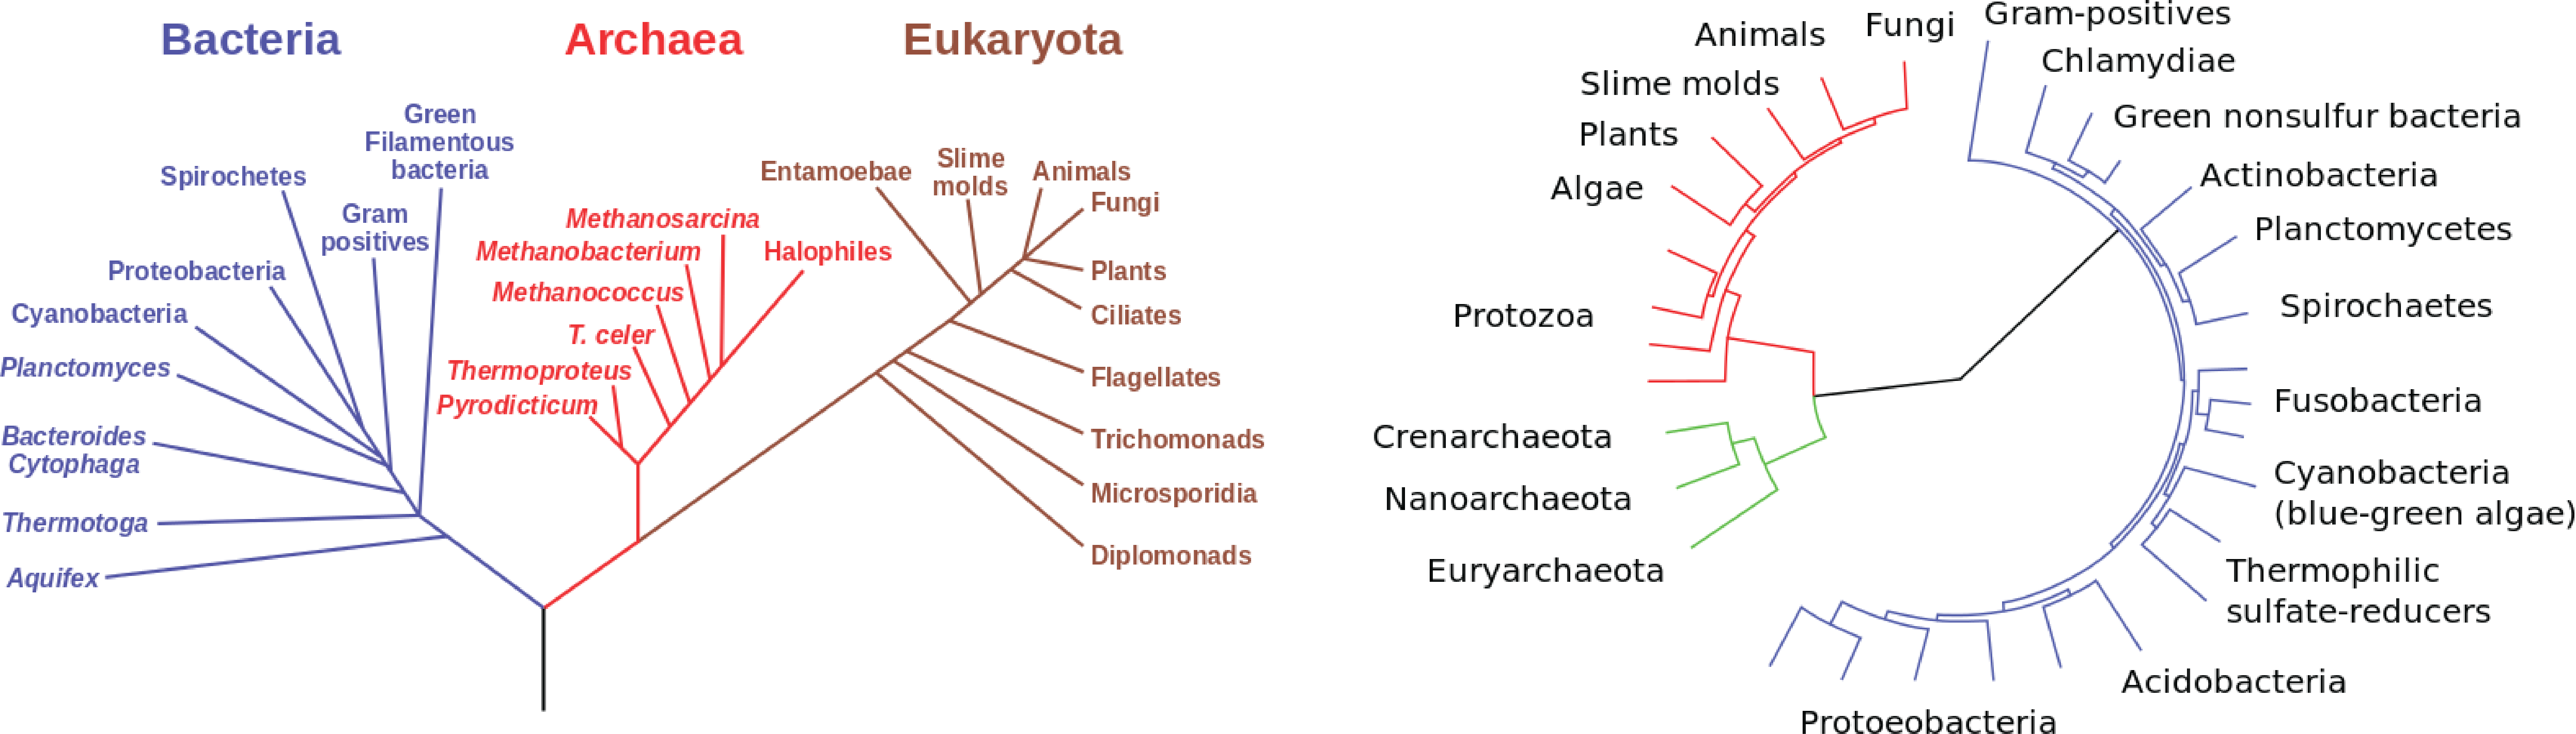
\includegraphics[width=0.75 \textwidth]{fig09/root_unroot_tree_example.png}
  \caption{Phylogenetic trees (sources: \href{https://commons.wikimedia.org/w/index.php?curid=9381199}{TimVickers, Wikimedia Commons}, \href{https://commons.wikimedia.org/w/index.php?curid=1201601}{NASA Astrobiology Institute, Wikimedia Commons}))}
\end{figure}

%
% Rooted and unrooted trees
%
\subsubsection*{Rooted and unrooted trees}
\begin{figure}[H]
  \centering
      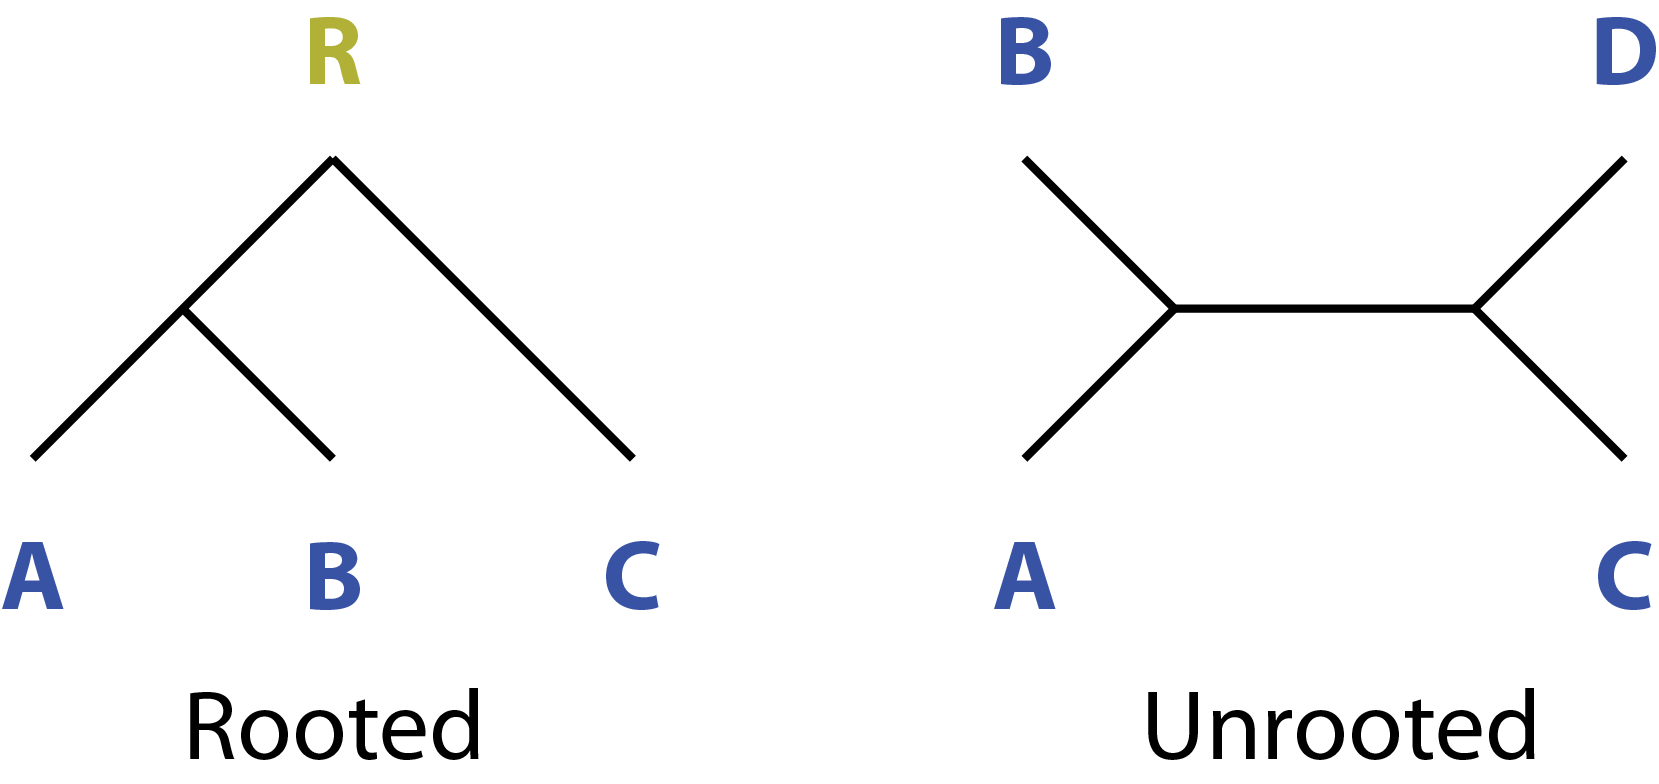
\includegraphics[width=0.35 \textwidth]{fig09/root_unroot_trees.png}
  \caption{A rooted tree with three nodes and an unrooted tree with four nodes}
\end{figure}

%
% Additive and ultrametric trees
%
\subsubsection*{Additive and ultrametric trees}
\begin{figure}[H]
  \centering
      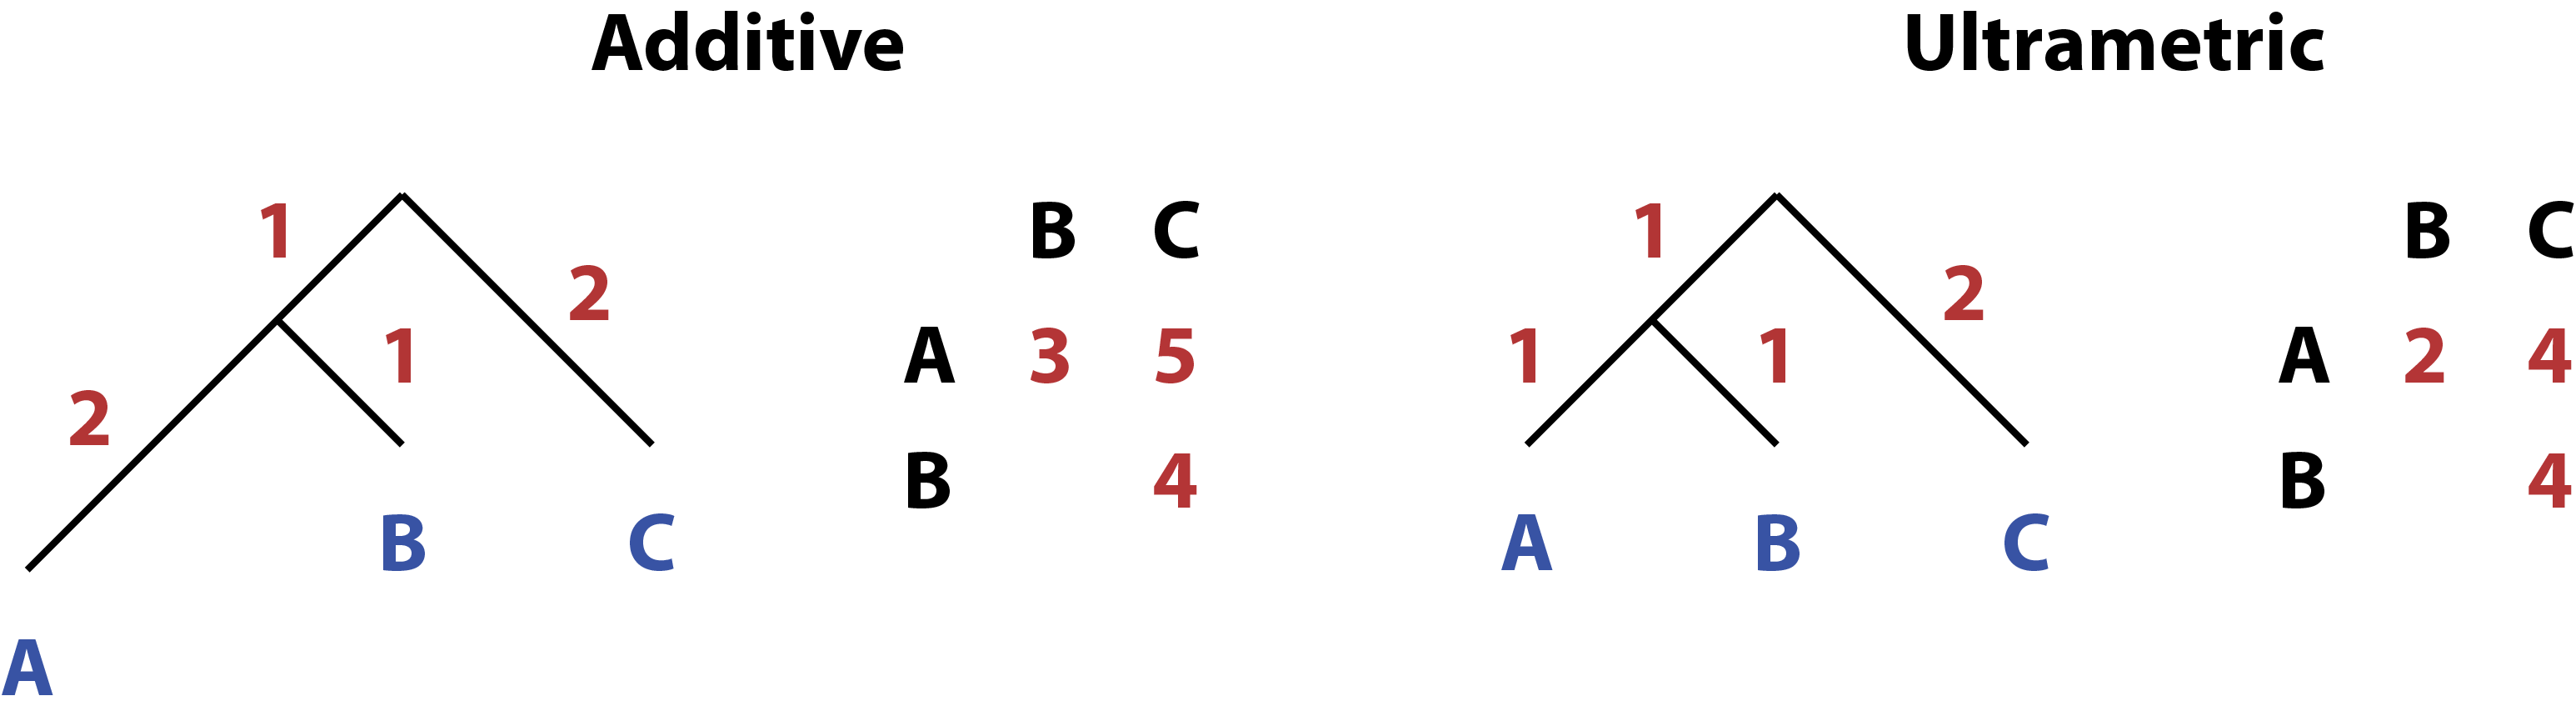
\includegraphics[width=0.6 \textwidth]{fig09/additive_ultrametric.png}
  \caption{A rooted tree with three nodes and an unrooted tree with four nodes}
\end{figure}
An ultrrametic tree is a special version of additive tree. It assumes that the distances from two sequences to their common ancestor are always equal.

%
% Number of topologically different tree
%
\subsubsection*{Number of topologically different tree}
\begin{figure}[H]
  \centering
      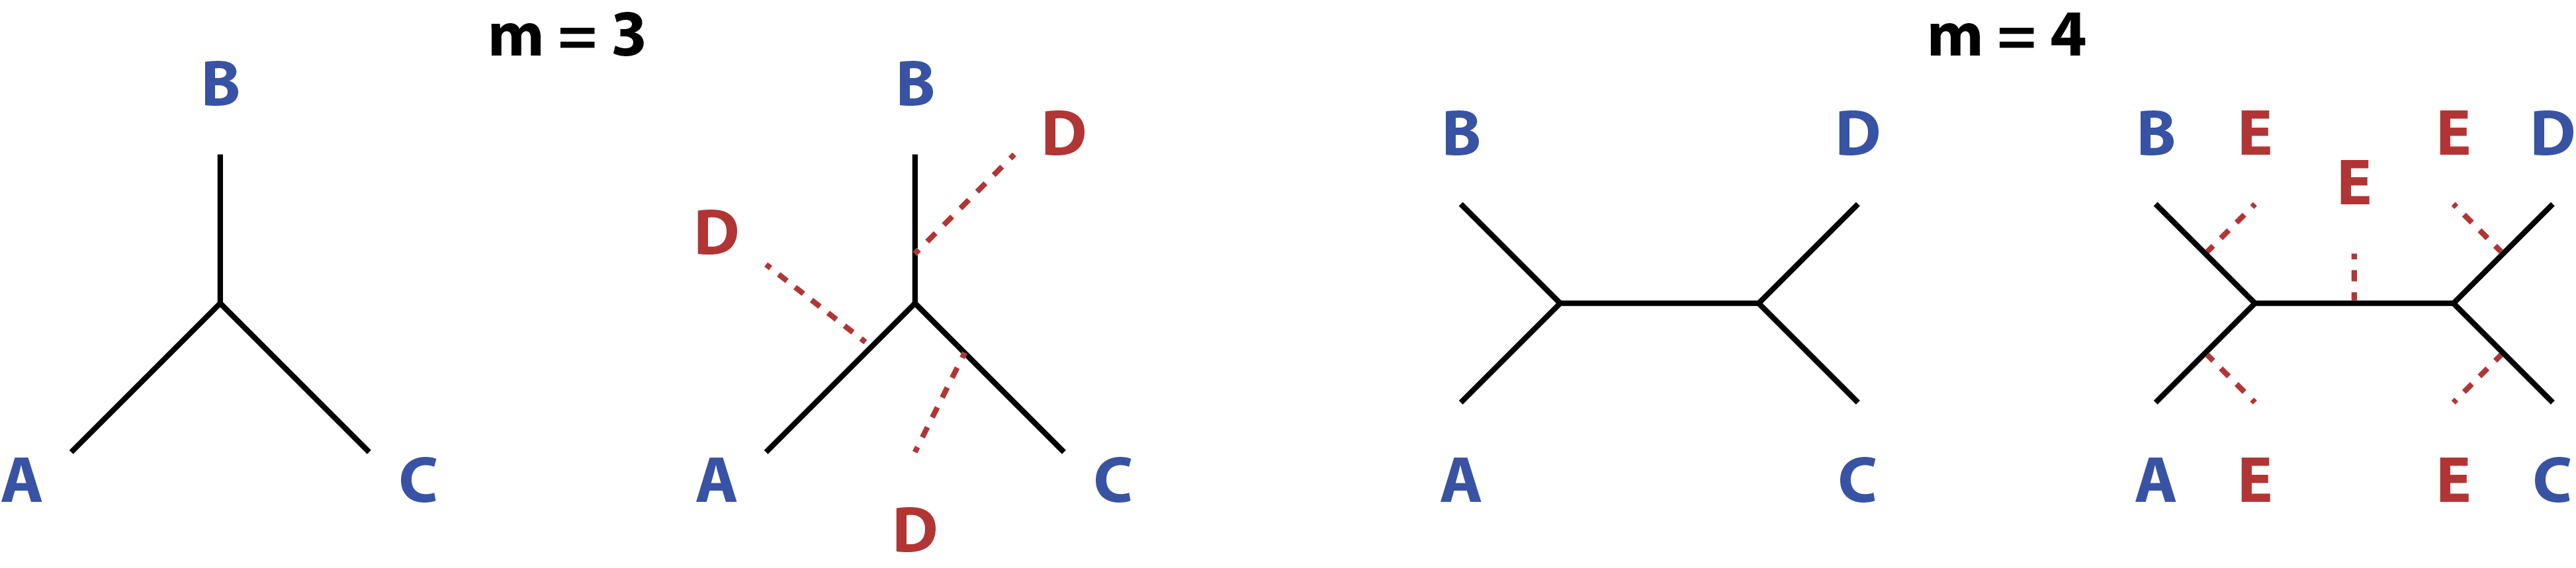
\includegraphics[width=0.7 \textwidth]{fig09/unroot_topology.png}
  \caption{Adding one external node to unrooted trees}
\end{figure}

The number of all possible topologically different unrooted tree $\mathrm{T_{unroot}}(m)$ can be obtained by the double factorial of $2m-5$.

\[
\mathrm{T_{unroot}}(m) = (2m - 5)!! \equiv \dfrac{(2m-5)!}{2^{m-3}(m-3)!}
\]
\medskip

\noindent
$\mathrm{T_{root}}(m)$ can be calculated from $\mathrm{T_{unroot}}(m)$. 

\[
\mathrm{T_{root}}(m) = (m-1) \times \mathrm{T_{unroot}}(m)
\]

%
% Example of the number of unrooted tree
%
\subsubsection*{Example of the number of unrooted tree}
What is the number of all possible topologically different unrooted trees when m = 7?

\[
\mathrm{T_{unroot}}(7) = (2 \times 7 - 5)!! = 9!! =1 \times 3 \times 5 \times 7 \times9 = 945
\]

or

\[
\mathrm{T_{unroot}}(7) = \dfrac{(2 \times 7 - 5)!}{2^{7-3}(7-3)!} = \dfrac{9!}{2^{4}(4)!} = 945
\]

%
% Exercise \thesection.1
%
\subsubsection*{Exercise \thesection.1}
\begin{enumerate}
\item Calculate the number of all possible topologically different unrooted trees when m = 5.
\medskip 

\item Construct an additive rooted tree for the distance matrix below. Estimate the edge values by trial and error.
\end{enumerate}

\begin{table}[H]
\centering
\begin{tabular}{|l|l|l|}
\hline
  & B & C \\ \hline
A & 4 & 7 \\ \hline
B &   & 5 \\ \hline
\end{tabular}
\end{table}

\bigskip 

%\end{document}
